The CE signal processing is implemented in application-specific integrated circuits (ASICs)
using CMOS technology.  The CE is continuously read out, resulting in a digitized ADC
sample from each APA channel (wire) up to every 500 ns (2~MHz sampling rate).

Each individual APA has 2,560 channels that are read out by 20 front-end motherboards (FEMBs), with
each FEMB providing digitized wire readout from 128 channels.  One cable bundle connects each FEMB to
the outside of the cryostat via a feedthrough (a CE feedthrough) in the signal cable flange at the
top of the cryostat, where a single flange services each APA, as shown in Figure~\ref{fig:connections}.
Each cable bundle contains wires for low-voltage (LV) power, high-speed data readout, and
clock/digital-control signal distribution.  Eight separate cables carry the TPC wire-bias voltages
from the signal flange to the APA wire-bias boards, in addition to the bias voltages for the field
cage termination electrodes and for the electron diverters.

\begin{dunefigure}
[Connections between the signal flanges and APA. Only the upper APA of the hanging APA pair, described in Section~\ref{sec:fdsp-apa-frames}, and its connection paths are shown. The lower APA will share the photodetector (PD) flange with the upper APA but have a separate TPC readout flange.]
{fig:connections}
{Connections between the signal flanges and APA. Only the upper APA of the hanging APA pair, described in Section~\ref{sec:fdsp-apa-frames}, and its connection paths are shown. The lower APA will share the photodetector (PD) flange with the upper APA but have a separate TPC readout flange.}
\hspace{1cm}
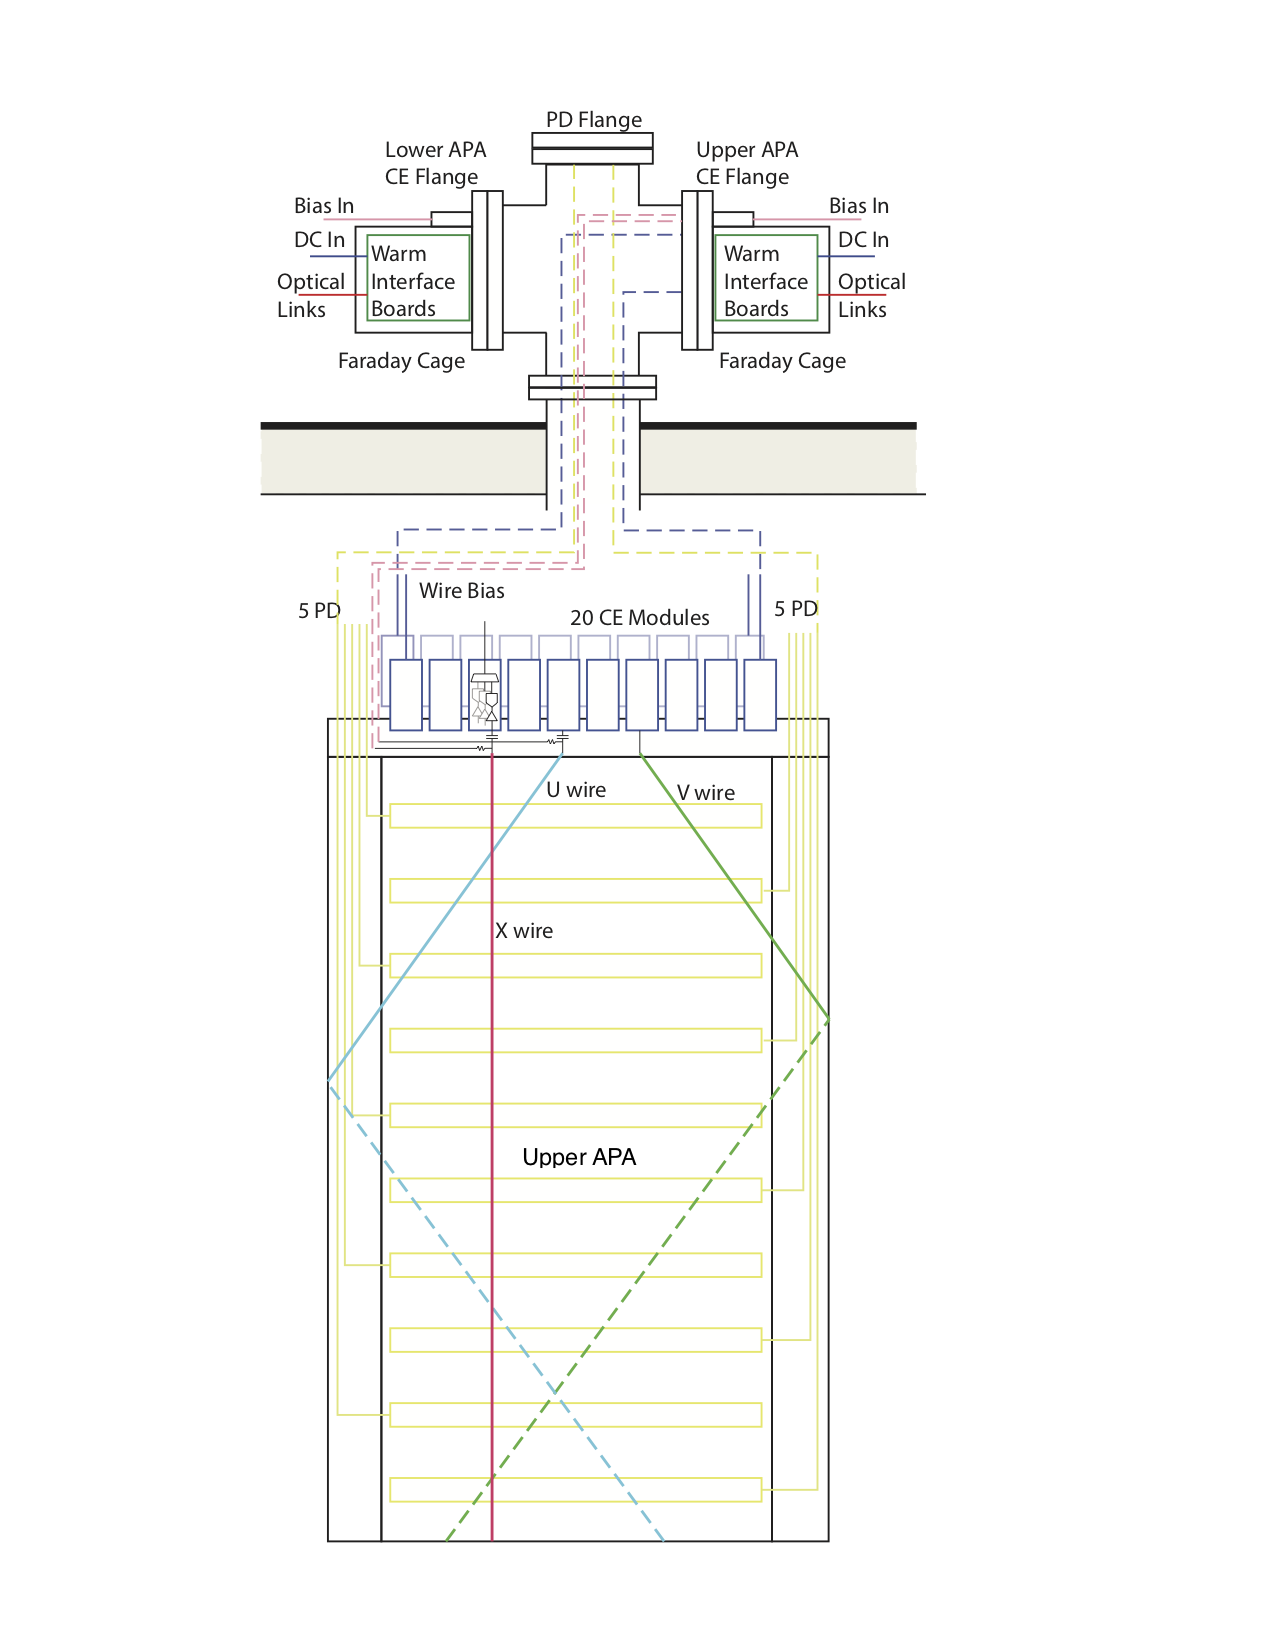
\includegraphics[width=0.9\textwidth]{tpcelec-PDSP_Connections.png}
\end{dunefigure}

The components of the CE system are the following:
\begin{itemize}
\item{FEMBs, which house the cold ASICs and are installed on the
APAs;}
\item{cables for the data, clock/control signals, LV power, and wire-bias voltages between the APA and the signal flanges (cold cables);}
\item{signal flanges with a CE feedthrough to pass the data, clock/control signals, LV power, and APA wire-bias voltages between the inside and outside of the cryostat, in addition to the corresponding cryostat penetrations and spool pieces;}
\item{warm interface electronics crates (WIECs) that are mounted on the signal flanges and contain
the warm interface boards (WIBs) and power and timing cards (PTCs) for further processing
and distribution of the signals entering/exiting the cryostat;}
%\item{fiber cables for transmitting data and clock/control signals between the WIECs and the
%data acquisition (DAQ) and slow control systems;}
\item{cables for LV power and wire-bias voltages between the signal flange and external power
supplies (warm cables); and}
\item{LV power supplies for the CE and bias-voltage power supplies for the APAs.}
\end{itemize}

The components, the quantity of each required for a single APA of the DUNE single-phase far detector, and the number of channels that each component has, are listed in Table~\ref{tab:elecNums}.

\begin{dunetable}
[TPC electronics components and quantities for a single APA of the DUNE single-phase far detector.]
{llr}
{tab:elecNums}
{TPC electronics components and quantities for a single APA of the DUNE single-phase far detector.}
\textbf{Element} &\textbf{Quantity} & \textbf{Channels per element}\\ \toprowrule
Front-end mother board (FEMB) & 20 per APA & 128 \\ \colhline
FE ASIC chip & 8 per FEMB & 16 \\ \colhline
ADC ASIC chip & 8 per FEMB & 16 \\ \colhline
COLDATA ASIC chip & 2 per FEMB & 64 \\ \colhline
Cold cable bundle & 1 per FEMB & 128 \\ \colhline
Signal flange & 1 per APA & 2,560 \\ \colhline
CE feedthrough & 1 per APA & 2,560 \\ \colhline
Warm interface board (WIB) & 5 per APA & 512 \\ \colhline
Warm interface electronics crate (WIEC) & 1 per APA & 2,560 \\ \colhline
Power and timing card (PTC) & 1 per APA & 2,560 \\ \colhline
Passive Backplane (PTB) & 1 per APA & 2,560 \\
%LV power mainframe & ? & ? \\ \colhline
%LV supply module & ? & ? \\ \colhline
%Wire-bias mini-crate & ? & ? \\ \colhline
%Wire-bias supply module & ? & ? \\
\end{dunetable}

The baseline design for the DUNE far detector single-phase TPC electronics calls for three types of ASICs to be located inside of the liquid argon:
\begin{itemize}
\item{a 16-channel front-end (FE) ASIC including amplification and pulse shaping, referred to as LArASIC in the following;}
\item{a 16-channel 12-bit ADC ASIC operating at 2~MHz; and}
\item{a 64-channel control and communications ASIC, referred to as COLDATA in the following.}
\end{itemize}
The FE ASIC has been prototyped and is close to meeting requirements (discussed in Section~\ref{sec:fdsp-tpc-elec-ov-req}). Another prototype to address issues in the version deployed in protoDUNE-SP is expected in Spring 2018. Key portions of the control and communications ASIC (also referred to as the COLDATA ASIC) have been prototyped and meet requirements.  However, it has been determined that the ``P1'' ADC ASIC now being used in protoDUNE-SP does not meet requirements, and accordingly, its development has been terminated.  A new cold ADC ASIC is being developed by an LBL-FNAL-BNL collaboration and first prototypes are expected by the end of Summer 2018.  The first full prototype of the controls and communication ASIC is also expected to be available for testing by the end of Summer 2018.  In order to maximize the probability of developing a complete design for cold TPC front-end electronics in a timely fashion, an alternative solution is also being investigated, a single 64-channel ASIC that will include all three functions described above.  This design is being done at SLAC and first prototypes are expected late in Spring 2018 or early Summer 2018.

While the higher charge carrier mobility at liquid argon temperature than at room temperature is central to the improved performance of cold electronics, it also leads to the ``hot carrier effect.''  In n-type MOS transistors, the carriers (electrons) can acquire enough kinetic energy to ionize silicon in the active channel.  This charge can become trapped and lead to effects (including threshold shifts) similar to those caused by radiation damage.  This effect can cause MOS circuits to ``age'' much more quickly at liquid argon temperature than at room temperature, reducing performance and potentially causing failure.  In order to mitigate this effect, the maximum electric field in transistor channels must be lower than the field that can be reliably used at room temperature.  This is accomplished by using transistors that are longer than minimum length and by using reduced bias voltage.  Any commercial circuits that are used in the liquid argon must be carefully tested to ensure that they will perform well for the expected 20-year lifetime of the DUNE.

A series of tests are planned to demonstrate that at least one of these designs will meet DUNE requirements. These include two system tests: one using the protoDUNE ``cold box'' at CERN, and one using a new small liquid argon TPC at Fermilab. The latter will also accommodate one half-length DUNE photodetector, and will provide a low noise environment that will allow one to make detailed comparisons of the performance of the new ASICs. It will also enable the study of interactions between the TPC readout and other systems, including the photodetector readout and the HV distribution.  These test facilities are discussed in more detail in Section~\ref{sec:fdsp-tpc-elec-qa-facilities}.
